\documentclass[12pt]{article}

\usepackage[a4paper, margin=1in]{geometry}
\usepackage{graphicx}
\usepackage{float}
\usepackage{hyperref}

\hypersetup{
    colorlinks=true,   
    urlcolor=cyan
}

\setlength\parindent{0pt}
\setlength\parskip{1em}

\title{System Architectures \\ \bigskip Centralized Chat System}
\author{\textsc{Nguyen} Duc Tung \\ ICT.M7.003}
\date{\textsc{Tran} Giang Son - \textsc{Daniel} Hagimont \\ \medskip
March 26$^{th}$, 2018}

\begin{document}

\maketitle

\section{Introduction}

In this project, I developed a functional IRC system, with the required architecture. I tried to prevent and handle as many runtime errors could happen as I can. The system supports broadcast in a channel, send private message (PM) to a specific client. It also provides commands for client and server to utilise the system. Both server and client work with multiplexed, nonblocking TCP socket connection.

There is a short clip (1:30 mins) that demo my system: \url{https://youtu.be/vtqJ2ZCUiHs}

\section{Client}

The client firstly takes server hostname from STDIN or from arguments, and then try to connect. After successfully connected, the program creates two separated threads: input handling thread, and network handling thread. Input thread send messages from keyboard to network thread through a pipe.

The pseudo design is as follows:

\begin{figure}[H]
\centering
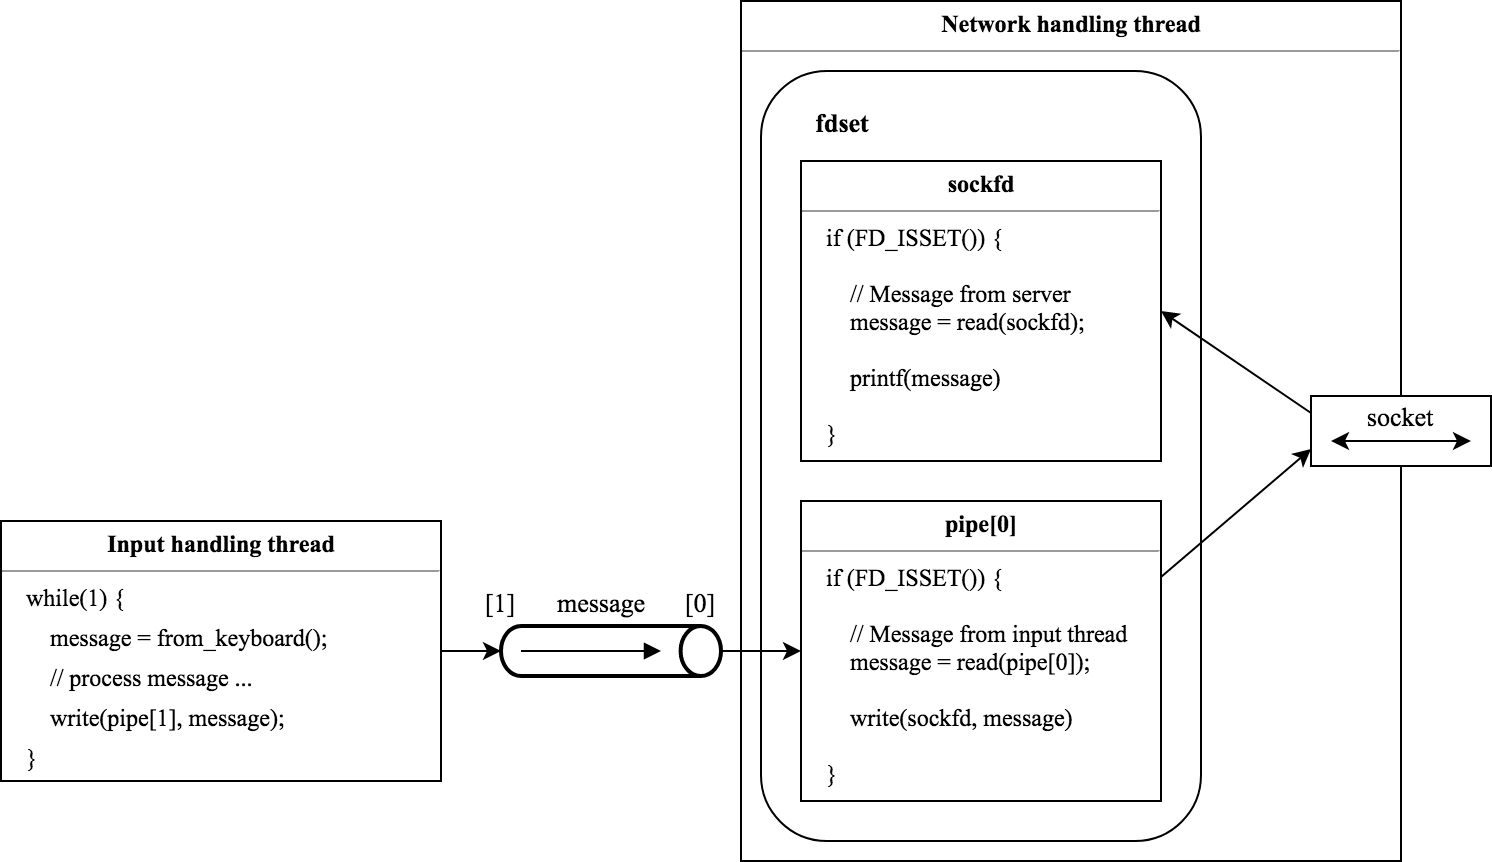
\includegraphics[width=\textwidth]{client_diagram.png}
\caption{Client's thread diagram}
\end{figure}

\subsection{Input handling thread}

The input handling thread continously getting message input from keyboard by user. The message runs through some processing such as remove `\textbackslash n' at the end, \dots After processed, message is sent to the pipe to be read by the network thread.

\subsection{Network handling thread}

The network handling thread have a \textbf{fdset} for multiplexed connection. The set include two file descriptors:

\begin{itemize}
\item \textbf{pipe[0]}: The read-end of the pipe between input thread and this thread. It is signaled when there are messages from the input thread. If the messages are successfully received, it will be send to the server.

\item \textbf{sockfd}: The socket file descriptor, it is signaled when there are messages from the server or when the connection is closed. If there are messages, it will be printed to the terminal. Otherwise, the program will stop.
\end{itemize}

\section{Server}

\subsection{Overall design}

The server will listen on a specific port for new connection. For each connection, it creates a child process to serve the client. A pair of pipe is used for each child process to communicate with the parent.

\begin{figure}[H]
\centering
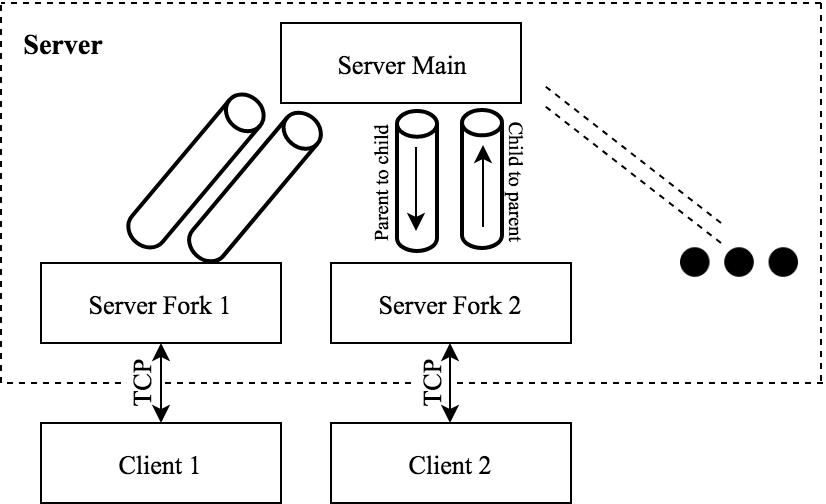
\includegraphics[width=0.75\textwidth]{server_diagram.png}
\caption{Server's design}
\end{figure}

\subsection{Main process}

When the server start, it will try to create a socket and listen for connections. The main process have an \textbf{fdset} including \textbf{STDIN}, \textbf{sockfd} (socket file descriptor), and \textbf{child\_to\_parent\_pipe[0]}(s)

\begin{itemize}
\item \textbf{STDIN}: The \textbf{STDIN} reads commands from the administrator, and process it. Details about the commands will be discussed later.

\item \textbf{sockfd}: Signaled when there are clients want to connect, it will accept if possible. After that, pipes will be setup and the server create a child process to handle it.

\item \textbf{child\_to\_parent\_pipe[0]}(s): These \textbf{pipes} signaled when there are messages from the child process (fundamentally from the client). The server will process the message. If it is a command, the command will be executed and response back the results to clients through \textbf{parent\_to\_child\_pipe[1]}(s). If it is a normal message, server will broadcast it to all connected clients (thorugh \textbf{pipes} with child process).
\end{itemize}

\subsection{Child processes}

Each child process also have a have an \textbf{fdset} including \textbf{parent\_to\_child\_pipe[1]}, and its \textbf{clientfd} (client file descriptor returned by \textit{accept()})

\begin{itemize}
\item \textbf{parent\_to\_child\_pipe[1]}: Signaled when there are messages from server to clients, just forward the message to its in-charged client.

\item \textbf{clientfd}: Signaled when trere are messages from the managing client. Simply send the messages to the server main process to handle.
\end{itemize}

\subsection{Client commands}

Following are supported commands for clients:

\begin{itemize}
\item \textbf{/help}: Show the help message to clients
\item \textbf{/id}: Show the clients their ID in the system
\item \textbf{/list}: List all connected clients
\item \textbf{/pm [destination ID] [message]}: Forward the message to only the desired client
\item \textbf{/quit}: Return the child process, disconnect the client, close the connection and the pipes setup before
\end{itemize}

\subsection{Server commands}

Following are supported commands for server:

\begin{itemize}
\item \textbf{help}: Show the help message for administrator
\item \textbf{list}: List all connected clients
\item \textbf{pm [client ID] [message]}: Send the message to a client
\item \textbf{broadcast [message]}: Broadcast the message to all connected clients
\item \textbf{dc [client ID]}: Disconnect a client
\item \textbf{shutdown}: Send a warning message to all clients, then close all the connections and shutdown server
\end{itemize}

\vfill
\centering\textit{That's the end of my report. Thank you for your consideration!}

\end{document}